\section{Unsupervised Language Model Pre-training}
The advent of unsupervised Language Model (LM) pre-training has led to significant performance gains on a variety of language understanding~\citep{radford2018improving,devlin-etal-2019-bert,yang2019xlnet,clark2020electra} and language generation~\citep{radford2019language,dong2019unified} tasks. Typically, a deep Long Shot-Term Memory networks (LSTM)~\citep{hochreiter1997long,peters-etal-2018-deep} or Transformer~\citep{vaswani2017attention} is first pre-trained on large-scale corpus and then the contextualized embeddings from the pre-trained language model are provided for the downstream tasks in the manner of feature extraction or fine-tuning.


\begin{sidewaysfigure}
    \centering
    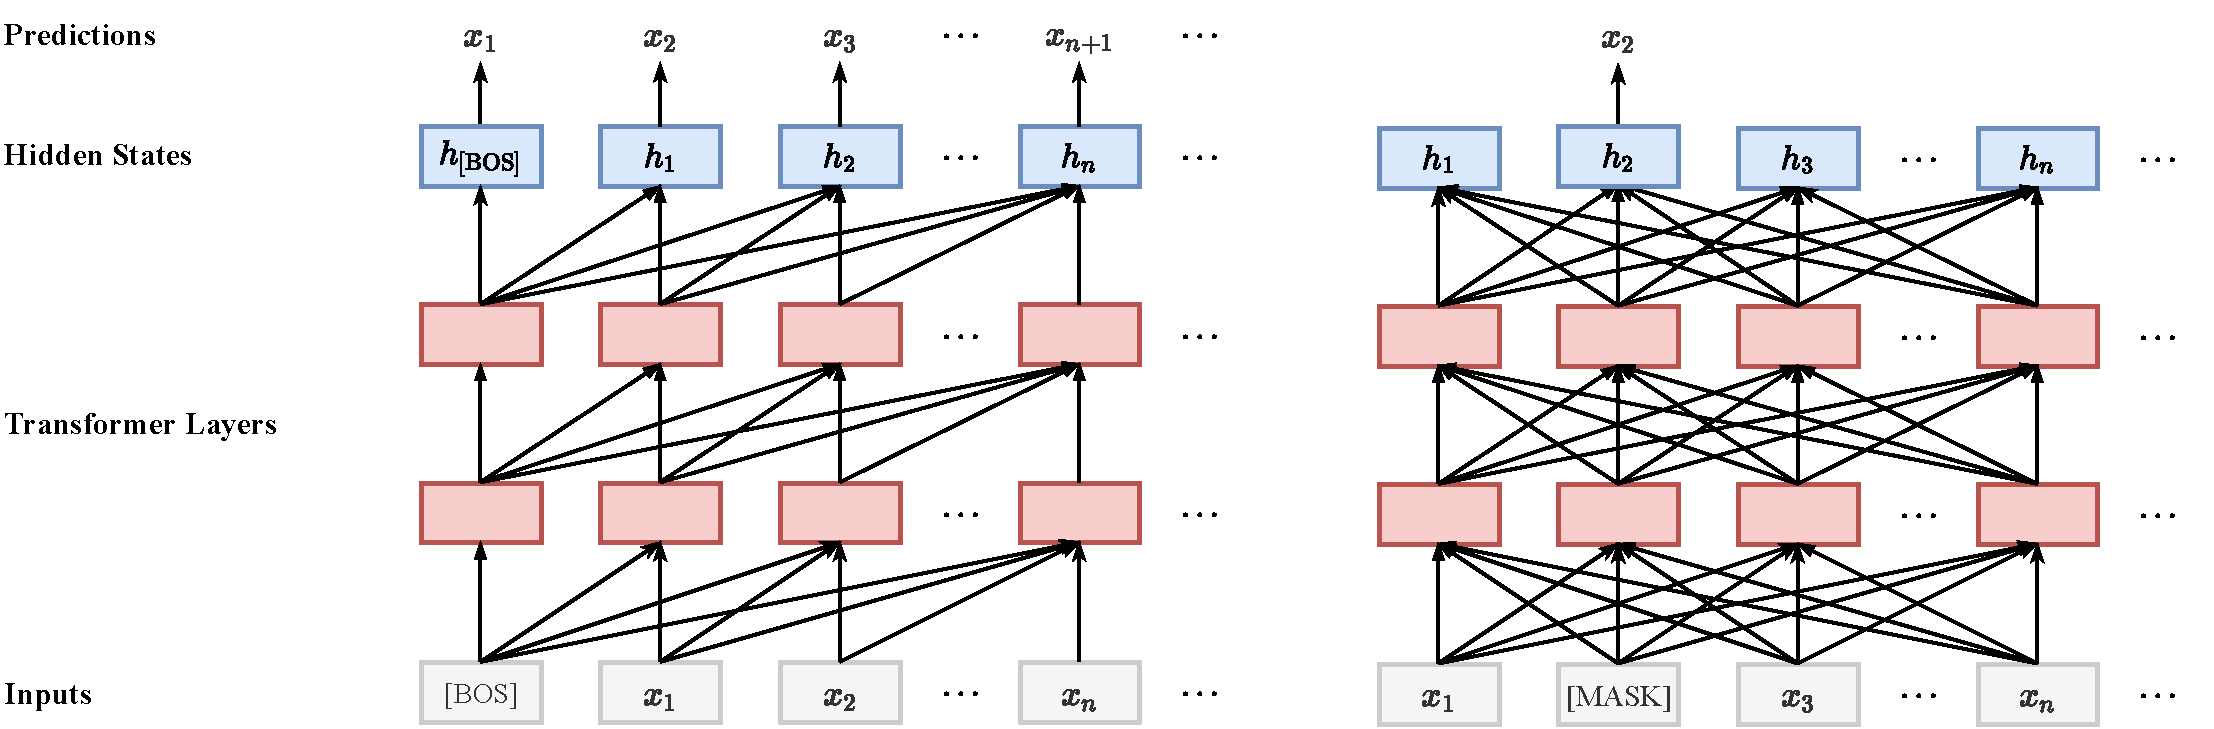
\includegraphics[width=\textwidth]{fig/ptlm.pdf}
    \caption{Auto-regressive language modeling (left) and masked language modeling (right).}
    \label{fig:ptlm}
\end{sidewaysfigure}

Several pre-training techniques have been developed for generating general-purpose contextualized embeddings. \citet{peters-etal-2017-semi,peters-etal-2018-deep} employ two unidirectional LSTM LMs, namely, a forward left-to-right LM and a backward right-to-left LM, to encode bi-directional contexts and the pre-training is conducted via auto-regressive language modeling, as shown in the left part of Figure~\ref{fig:ptlm}. GPT~\citep{radford2018improving} and GPT-2~\citep{radford2019language} adopt the same auto-regressive pre-training objective but change to model sequential word flow with unidirectional Transformer. BERT~\citep{devlin-etal-2019-bert}, as well as its variants~\citep{conneau2019cross,liu2019roberta,wang2019structbert,joshi-etal-2020-spanbert}, propose to learn contextualized embeddings based on masked language modeling---reconstruct the masked input with the special \texttt{[MASK]} token and the surrounding context (see the right part of Figure~\ref{fig:ptlm}). In order to unify the auto-regressive pre-training and auto-encoding based pre-training, UniLM~\citep{dong2019unified} jointly optimizes the pre-training of Transformer with auto-regressive language modeling objective and masked language modeling objective. Similarly, XLNet~\citep{yang2019xlnet} designs permutation language modeling objective to capture the context information from all positions while preserving the temporal dependency among the predictions. MASS~\citep{song2019mass}, BART~\citep{lewis-etal-2020-bart} and T5~\citep{raffel2019exploring} are the initial attempts to pre-train sequence-to-sequence architecture and achieve promising results on machine translation and abstractive summarization. 


\section{Multilingual Language Model Pre-Training}
Multilingual language model pre-training is a multilingual extension of language model pre-training, where the deep neural architecture~\citep{vaswani2017attention,peters-etal-2018-deep} is pre-trained on large-scale multilingual corpus, e.g., a collection of wikipedia documents in different languages. The yielding multilingual pre-trained language models (mPTLMs)~\citep{che-etal-2018-towards,devlin-etal-2019-bert,conneau2019cross,mulcaire-etal-2019-polyglot,conneau-etal-2020-unsupervised} have been regarded as the gold standard for a variety of unsupervised cross-lingual natural language understanding tasks~\citep{prettenhofer-stein-2010-cross,schwenk-li-2018-corpus,zeman-etal-2018-conll,liu-etal-2019-xqa}. The most impressive features of mPTLMs is that even performing cross-lingual transfer in a zero-shot manner---only fine-tune the mPTLMs on the source-language training data---it can still significantly outperform the existing works based on cross-lingual embeddings~\citep{mikolov2013exploiting,faruqui-dyer-2014-improving,smith2018offline} or machine translation~\citep{banea-etal-2008-multilingual,duh-etal-2011-machine}, as observed in~\citet{pires-etal-2019-multilingual,wu-dredze-2019-beto,keung-etal-2019-adversarial,artetxe-etal-2020-cross}. After being additionally trained on machine-translated data from source language, the cross-lingual performances of the cross-lingual models exploiting mPTLMs are further improved~\citep{huang-etal-2019-unicoder,conneau-etal-2020-unsupervised,cao2020multilingual}, especially on sequence classification~\citep{schwenk-li-2018-corpus} and sequence pair classification tasks~\citep{conneau-etal-2018-xnli,yang-etal-2019-paws}.
